The \gls{EPICS} and related toolkits can be used to control large experiments or even beamlines, but also smaller experimental setups, in which only limited functionalities are needed. During the R\&D phase for the \gls{STS} many different setups were constructed, in order to evaluate the hardware that should be used for the final experiment. Moreover, challenging ambient conditions of the \gls{STS} put even more stringent constraints. To address the needs of this dynamic environment, a container-based control framework was implemented. 
The two following sections introduce the applications of the developed software package for effective control and data acquisition in two chosen setups. The first of mentioned sections focuses on the powering units irradiation studies and implications for the \gls{STS}. The last section discusses the results from the thermal cycling activities for the \gls{STS} electronics, which aimed to discover their operational limitations. 

\section{Monitoring of the Frond End Electronics}
The first application of the introduced control framework was to read out several parameters from different readout chains (see section \ref{readout} for a detailed explanation of different readout chains). The \gls{ROB} and \gls{DPB} based readout chain was mostly used to evaluate the possibility of interfacing the values from the \gls{DAQ} chain to the slow control and \gls{EPICS} based system. The purpose, similarly to the GBTxEMU chain, was to monitor the stability of the readouts throughout different tests, e.g. thermal cycling of the \gls{FEE}. A maximum of 2 \glspl{FEB} - 16 STS-XYTERs were used, so in total 112 process variables were monitored, which makes it a small setup. Those values were then stored in a database and are available from Phoebus. 

The available parameters included those available from \gls{GBT} \gls{SCA2} \gls{ASIC} \cite{GBT_SCA_ASIC} and three GBTX chips: 
\begin{itemize}
    \item GBT SCA - RSSI (Received Single Strength Indicator), Input voltage $V_{in}$, 1.5V DC/DC converter output voltage $V_{out}$, 2.5V DC/DC converter output voltage $V_{out}$ (see figure~\ref{fig:ROB}), two temperature sensors,
    \item GBTX \gls{ASIC} - FEC (Forward Error Correction) counts.
\end{itemize}
%\newpage

\begin{figure}[!h]
    \centering
    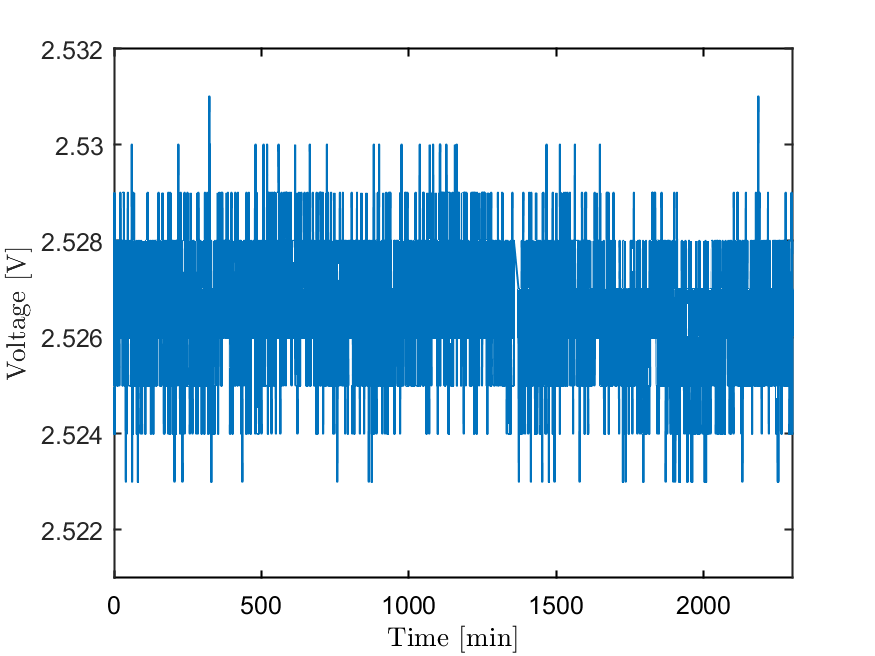
\includegraphics[width=0.65\columnwidth]{Chapter4/images/ROB.png}
    \caption{$V_{out}$ output voltage from one of the DC/DC converters in the \gls{ROB}}
    \label{fig:ROB}
\end{figure}

The STS-XYTER provides the following values - almost full counter, event missed counter, single event upset counter, the status register, and \gls{DAC} values: $V_{ddm}$, \gls{CSA} bias, temperature. 

\begin{figure}[!h]
    \centering
    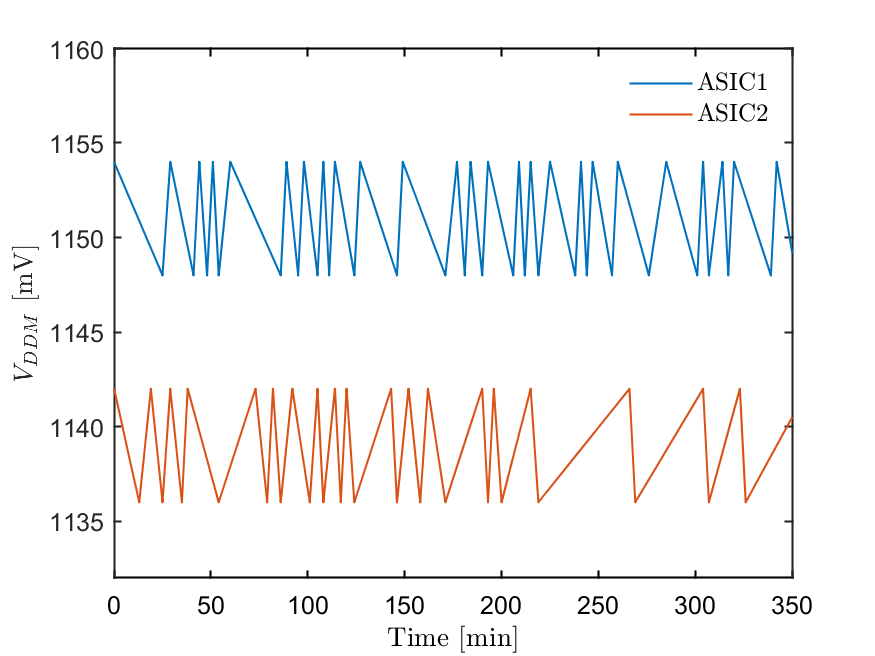
\includegraphics[width=0.65\columnwidth]{Chapter4/images/FEB.png}
    \caption{$V_{ddm}$ readouts from the diagnostic circuits of two ASICs}
    \label{fig:vddm_first}
\end{figure}

FEE monitoring plays a crucial role in the detector operation but also during the testing phase. Internal parameters of the ASICs in the \gls{ROB} or \gls{FEB} deliver information about the stability and onset of failure. %\subsection{Parameters of the STS-XYTERv2 ASIC}
%\subsection{GBTX and GBT ASIC monitoring}